\section{\textit{Review} expresso de variedades}
\label{sec: 2}
Antes de definir nosso principal objeto de estudo, temos que entender os conceitos da Geometria Diferencial. Aqui obviamente só temos o mínimo consolidado de modo que este seja o mais auto contido possível, porém, uma ótima referência para se nortear esta contemplada nas Notas de Aula de Geometria Riemanniana \cite{malex2022} ou também em \cite{munkres2018analysis}. 

\subsection{Variedades suaves}

Como base, temos que definir os espaços com os quais iremos trabalhar:

\begin{definicao}[Variedade Topológica]
	Um espaço topológico $M$ é uma \textit{variedade topológica de dimensão} $n$ se as seguintes condições forem satisfeitas:
	\begin{enumerate}
		\item $M$ é Hausdorff;
		\item $M$ é segundo contável, ou seja, possui uma base enumerável;
		\item $M$ é localmente euclidiano de dimensão $n$, isto é, todo ponto de $M$ possui uma vizinhança homeomorfa a um aberto de $\mathbb R^n$.
	\end{enumerate}
\end{definicao}

No item 3 acima, se $U$ é a vizinhança em questão e $\phi: U \longrightarrow \mathbb R^n$ é um homeomorfismo entre $U$ e um aberto $\phi(U) \subseteq \mathbb R^n$, chamamos o par $(U, \phi)$ de \textit{carta coordenada}. No nosso caso, a variedade topológica representa intuitivamente o que vemos como curvas e superfícies em $\mathbb R^3$, mas precisaremos muni-la com alguma estrutura diferenciável para podermos trabalhar melhor. Transportaremos o cálculo diferencial de $\mathbb R^n$ para a variedade através das cartas coordenadas.

\begin{definicao}[Mudança de Coordenadas]
	Duas cartas $(U, \varphi: U \longrightarrow \mathbb R^n)$, $(V, \psi: V \longrightarrow \mathbb R^n)$ de uma variedade topológica são $C^{\infty}$-\textit{compatíveis} se os \textit{mapas de transição}
	\[
	\varphi \circ \psi^{-1}: \psi(U \cap V) \longrightarrow \varphi(U \cap V), \quad \psi \circ \varphi^{-1}: \varphi(U \cap V) \longrightarrow \psi(U \cap V)
	\]
	são $C^{\infty}$. Esses também podem ser chamados de \textit{mudanças de coordenadas}.
	\begin{figure}[H]
		\centering
		

\tikzset{every picture/.style={line width=0.45pt}} %set default line width to 0.75pt        

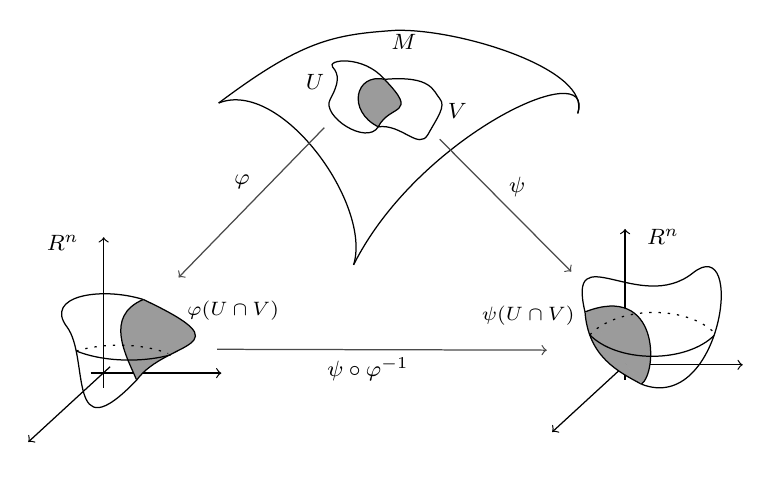
\begin{tikzpicture}[x=0.75pt,y=0.75pt,yscale=-1,xscale=1]
%uncomment if require: \path (0,300); %set diagram left start at 0, and has height of 300

%Curve Lines [id:da12253634132608959] 
\draw    (130.5,61) .. controls (160.5,49) and (204.5,110) .. (195.5,139) ;
%Curve Lines [id:da09568098876338671] 
\draw    (195.5,139) .. controls (226.5,77) and (312.5,37) .. (303.5,66) ;
%Curve Lines [id:da12952951962291093] 
\draw    (130.5,61) .. controls (170.5,31) and (185.5,28) .. (215.5,26) ;
%Curve Lines [id:da8017459310615034] 
\draw    (215.5,26) .. controls (246.5,25) and (310.5,45) .. (303.5,66) ;
%Straight Lines [id:da11165753602356343] 
\draw [color={rgb, 255:red, 74; green, 74; blue, 74 }  ,draw opacity=1, -> ]   (181.4,72.86) -- (111.19,145.03) ;
%\draw [shift={(109.8,146.46)}, rotate = 314.21000000000004] [color={rgb, 255:red, 74; green, 74; blue, 74 }  ,draw opacity=1 ][line width=0.75]    (10.93,-3.29) .. controls (6.95,-1.4) and (3.31,-0.3) .. (0,0) .. controls (3.31,0.3) and (6.95,1.4) .. (10.93,3.29) ;
%Shape: Axis 2D [id:dp8820201499438707] 
\draw[->]  (68.8,191.13) -- (131.8,191.13);
\draw[<-] (75.1,125.66) -- (75.1,198.4);
%Straight Lines [id:da7817199884965225] 
\draw[->]  (78.2,188.06) -- (38.78,224.31) ;
%\draw [shift={(37.3,225.67)}, rotate = 317.4] [color={rgb, 255:red, 0; green, 0; blue, 0 }  ][line width=0.75]    (10.93,-3.29) .. controls (6.95,-1.4) and (3.31,-0.3) .. (0,0) .. controls (3.31,0.3) and (6.95,1.4) .. (10.93,3.29)   ;
%Straight Lines [id:da21051464502306283] 
\draw [color={rgb, 255:red, 74; green, 74; blue, 74 }  ,draw opacity=1, ->]   (237,78.46) -- (300.39,142.24) ;
%\draw [shift={(301.8,143.66)}, rotate = 225.18] [color={rgb, 255:red, 74; green, 74; blue, 74 }  ,draw opacity=1 ][line width=0.75]    (10.93,-3.29) .. controls (6.95,-1.4) and (3.31,-0.3) .. (0,0) .. controls (3.31,0.3) and (6.95,1.4) .. (10.93,3.29)   ;
%Shape: Axis 2D [id:dp22295758051907422] 
\draw[->]  (320,187.13) -- (383,187.13);
\draw[<-] (326.3,121.66) -- (326.3,194.4);
%Straight Lines [id:da3563469474596257] 
\draw[->]    (330.6,183.26) -- (291.18,219.51) ;
%\draw [shift={(289.7,220.87)}, rotate = 317.4] [color={rgb, 255:red, 0; green, 0; blue, 0 }  ][line width=0.75]    (10.93,-3.29) .. controls (6.95,-1.4) and (3.31,-0.3) .. (0,0) .. controls (3.31,0.3) and (6.95,1.4) .. (10.93,3.29)   ;
%Straight Lines [id:da572071933187088] 
\draw [color={rgb, 255:red, 155; green, 155; blue, 155 }  ,draw opacity=1 ][fill={rgb, 255:red, 155; green, 155; blue, 155 }  ,fill opacity=1 ]   (94.2,155.66) -- (91,194.46) ;
%Straight Lines [id:da18438752078564646] 
\draw [color={rgb, 255:red, 155; green, 155; blue, 155 }  ,draw opacity=1 ][fill={rgb, 255:red, 155; green, 155; blue, 155 }  ,fill opacity=1 ]   (307,161.66) -- (331.8,193.66) ;
%Curve Lines [id:da951001718333709] 
\draw    (307,161.66) .. controls (298.2,124.46) and (333.4,163.26) .. (359,142.86) .. controls (384.6,122.46) and (373,211.66) .. (334.2,196.46) ;
%Curve Lines [id:da19213944484530643] 
\draw    (91,194.46) .. controls (56.6,230.46) and (68.6,183.66) .. (57.4,168.86) .. controls (46.2,154.06) and (73.4,149.26) .. (94.2,155.66) ;
%Straight Lines [id:da3787366607544964] 
\draw [color={rgb, 255:red, 74; green, 74; blue, 74 }  ,draw opacity=1, ->]   (129.8,179.66) -- (288.6,180.06) ;
%\draw [shift={(290.6,180.06)}, rotate = 180.14] [color={rgb, 255:red, 74; green, 74; blue, 74 }  ,draw opacity=1 ][line width=0.75]    (10.93,-3.29) .. controls (6.95,-1.4) and (3.31,-0.3) .. (0,0) .. controls (3.31,0.3) and (6.95,1.4) .. (10.93,3.29)   ;
%Curve Lines [id:da24270644855795598] 
\draw    (210.4,49.6) .. controls (233.4,47.66) and (233.8,55.26) .. (237,58.86) .. controls (240.2,62.46) and (235.8,68.06) .. (231.4,76.06) .. controls (227,84.06) and (218.69,70.89) .. (207.4,72.46) ;
%Curve Lines [id:da33545782983962047] 
\draw    (210.4,49.6) .. controls (200.2,37.66) and (182.2,40.06) .. (185.4,43.66) .. controls (188.6,47.26) and (188.6,51.26) .. (184.2,59.26) .. controls (179.8,67.26) and (201.8,81.66) .. (207.4,72.46) ;
%Straight Lines [id:da14052521632408] 
\draw [color={rgb, 255:red, 155; green, 155; blue, 155 }  ,draw opacity=1 ][fill={rgb, 255:red, 155; green, 155; blue, 155 }  ,fill opacity=1 ]   (210.4,49.6) -- (207.4,72.46) ;
%Curve Lines [id:da2501449241188438] 
\draw [fill={rgb, 255:red, 155; green, 155; blue, 155 }  ,fill opacity=1 ]   (207.4,72.46) .. controls (192.2,64.86) and (196.2,46.46) .. (210.4,49.6) ;
%Curve Lines [id:da2598296067011632] 
\draw [fill={rgb, 255:red, 155; green, 155; blue, 155 }  ,fill opacity=1 ]   (210.4,49.6) .. controls (227.4,67.26) and (213,61.26) .. (207.4,72.46) ;
%Curve Lines [id:da5220380098580575] 
\draw [fill={rgb, 255:red, 155; green, 155; blue, 155 }  ,fill opacity=1 ]   (91,194.46) .. controls (85.8,182.46) and (75.19,163.72) .. (94.2,155.66) ;
%Curve Lines [id:da5783963299572314] 
\draw [fill={rgb, 255:red, 155; green, 155; blue, 155 }  ,fill opacity=1 ]   (94.2,155.66) .. controls (145,179.66) and (105.4,174.86) .. (91,194.46) ;
%Shape: Arc [id:dp7983026148871659] 
\draw  [draw opacity=0] (107.37,182.33) .. controls (101.59,183.93) and (94.75,184.85) .. (87.41,184.85) .. controls (77.56,184.85) and (68.6,183.19) .. (61.92,180.47) -- (87.41,168.52) -- cycle ; \draw   (107.37,182.33) .. controls (101.59,183.93) and (94.75,184.85) .. (87.41,184.85) .. controls (77.56,184.85) and (68.6,183.19) .. (61.92,180.47) ;
%Shape: Arc [id:dp4531975717042873] 
\draw  [draw opacity=0][dash pattern={on 0.84pt off 2.51pt}] (61.92,180.47) .. controls (67.6,178.76) and (74.39,177.74) .. (81.69,177.68) .. controls (91.08,177.6) and (99.66,179.12) .. (106.14,181.69) -- (81.83,194.01) -- cycle ; \draw  [dash pattern={on 0.84pt off 2.51pt}] (61.92,180.47) .. controls (67.6,178.76) and (74.39,177.74) .. (81.69,177.68) .. controls (91.08,177.6) and (99.66,179.12) .. (106.14,181.69) ;
%Curve Lines [id:da40298571757933943] 
\draw [fill={rgb, 255:red, 155; green, 155; blue, 155 }  ,fill opacity=1 ]   (334.2,196.46) .. controls (323,190.46) and (308.6,183.26) .. (307,161.66) ;
%Curve Lines [id:da8319827009641485] 
\draw [fill={rgb, 255:red, 155; green, 155; blue, 155 }  ,fill opacity=1 ]   (307,161.66) .. controls (342.79,147.52) and (342.2,190.46) .. (334.2,196.46) ;
%Shape: Arc [id:dp5999943800568168] 
\draw  [draw opacity=0] (369.2,172.96) .. controls (363.26,178.98) and (352.14,183.03) .. (339.4,183.03) .. controls (326.46,183.03) and (315.19,178.85) .. (309.32,172.67) -- (339.4,162.9) -- cycle ; \draw   (369.2,172.96) .. controls (363.26,178.98) and (352.14,183.03) .. (339.4,183.03) .. controls (326.46,183.03) and (315.19,178.85) .. (309.32,172.67) ;
%Shape: Arc [id:dp7315027451637988] 
\draw  [draw opacity=0][dash pattern={on 0.84pt off 2.51pt}] (309.32,172.67) .. controls (315.13,166.52) and (326.15,162.21) .. (338.88,161.92) .. controls (351.82,161.63) and (363.18,165.55) .. (369.2,171.59) -- (339.34,182.05) -- cycle ; \draw  [dash pattern={on 0.84pt off 2.51pt}] (309.32,172.67) .. controls (315.13,166.52) and (326.15,162.21) .. (338.88,161.92) .. controls (351.82,161.63) and (363.18,165.55) .. (369.2,171.59) ;

% Text Node
\draw (171.2,45.8) node [anchor=north west][inner sep=0.75pt]  [font=\footnotesize]  {$U$};
% Text Node
\draw (239.6,60) node [anchor=north west][inner sep=0.75pt]  [font=\footnotesize]  {$V$};
% Text Node
\draw (136.8,94.2) node [anchor=north west][inner sep=0.75pt]  [font=\footnotesize]  {$\varphi $};
% Text Node
\draw (269.2,95.2) node [anchor=north west][inner sep=0.75pt]  [font=\footnotesize]  {$\psi $};
% Text Node
\draw (114,155.2) node [anchor=north west][inner sep=0.75pt]  [font=\scriptsize]  {$\varphi ( U\cap V)$};
% Text Node
\draw (256,157.6) node [anchor=north west][inner sep=0.75pt]  [font=\scriptsize]  {$\psi ( U\cap V)$};
% Text Node
\draw (181.6,182.4) node [anchor=north west][inner sep=0.75pt]  [font=\footnotesize]  {$\psi \circ \varphi ^{-1}$};
% Text Node
\draw (46.4,123.6) node [anchor=north west][inner sep=0.75pt]  [font=\footnotesize]  {$\mathbb{R}^{n}$};
% Text Node
\draw (335.6,120.4) node [anchor=north west][inner sep=0.75pt]  [font=\footnotesize]  {$\mathbb{R}^{n}$};
% Text Node
\draw (212.4,26.6) node [anchor=north west][inner sep=0.75pt]  [font=\footnotesize]  {$M$};


\end{tikzpicture}

		\caption{Ilustração de uma mudança de coordenadas}
		\label{fig: troca de coordenadas}
	\end{figure}
\end{definicao}


Veja que os mapas de transição acima são homeomorfismos entre abertos de $\mathbb R^n$, logo faz sentido verificar se eles são suaves. Passando essa definição ao global:

\begin{definicao}[Atlas]
	Um \textit{atlas} $C^{\infty}$ numa variedade topológica $M$ é uma coleção $\{(U_{\alpha}, \phi_{\alpha}) \mid \alpha \in \LLambda\}$ de cartas coordenadas duas a duas $C^{\infty}$-compatíveis que cobrem $M$, ou seja, $M = \bigcup_{\alpha\in \LLambda} U_{\alpha}$.
\end{definicao}

Estamos quase lá! Poderíamos dizer que uma variedade suave é uma variedade topológica que possui um atlas $C^{\infty}$. O problema é que quando dois atlas diferentes são compatíveis entre si, eles essencialmente carregam a mesma informação. Dessa forma, queremos unir todos os atlas que são ``equivalentes''. Com essa ideia, não é difícil provar que todo atlas está contido em um único atlas $C^{\infty}$ \textit{maximal}, ou seja, que não está propriamente contido em nenhum outro atlas. Agora sim estamos prontos!

\begin{definicao}[Variedade Suave]
	Uma \textit{variedade suave} é uma variedade topológica juntamente com um atlas $C^{\infty}$ maximal.
\end{definicao}

Boa parte das propriedades de diferenciabilidade se traduzem localmente para o contexto de variedades suaves através das cartas coordenadas. Por exemplo, podemos definir funções suaves entre variedades. Diremos que uma função $F: N \longrightarrow M$ entre variedades suaves é $C^{\infty}$ em um ponto $p \in N$ se existem cartas coordenadas $(U, \phi)$ sobre $p$ e $(V, \psi)$ sobre $F(p)$ tais que $\psi \circ F \circ \phi^{-1}$ é uma função $C^{\infty}$ em $\phi(p)$. Não é difícil mostrar que, para outras cartas sobre $p$ e $F(p)$, a função induzida entre abertos de $\mathbb R^n$ e $\mathbb R^m$ ainda é suave no ponto em questão. Assim, nossa definição faz sentido. Nesse caso, $F$ será suave se for $C^{\infty}$ em todo ponto.

Por fim, um conceito muito importante nessa linha é o de difeomorfismo. Uma função $F: N \longrightarrow M$ entre variedades suaves é um \textit{difeomorfismo} se for suave, bijetora e tiver inversa suave. Duas variedades \textit{difeomorfas} são essencialmente a mesma no quesito da diferenciabilidade. 

\subsection{O Espaço Tangente}
\label{sec:O espaco Tangente}
Para definir formas e uma teoria de integração em variedades, é imprescindível definir o espaço tangente e discutir suas propriedades. No caso mais visual de variedades mergulhadas em $\mathbb R^2$ ou $\mathbb R^3$, intuitivamente vemos o espaço tangente em um ponto $p$ da variedade como sendo o conjunto dos vetores que são tangentes a curvas suaves que passam por $p$. Porém, como estamos adotando uma definição mais abstrata e geral, não é tão claro qual seria uma boa definição. O que se segue é uma abordagem diferente, que equivale à definição mais visual, nos casos onde ambas se aplicam.

Definimos um \textit{germe} de uma função $C^\infty$ em um ponto $p$ de uma variedade $M$ como a classe de equivalência de funções $C^{\infty}$ definidas numa vizinhança de $p$ em $M$, sendo duas funções equivalentes se elas concordam numa vizinhança (possivelmente menor) de $p$. O conjunto desses germes em $p$ será denotado por $C^{\infty}_p(M)$. Note que $C^{\infty}_p(M)$ é um espaço vetorial. Chamaremos de \textit{derivação em um ponto} $p$ numa variedade $M$ um mapa linear $D: C^{\infty}_p(M) \longrightarrow \mathbb R$ que satisfaz a ``Regra de Leibniz'':
\begin{equation*}
	D(fg) = (Df)g(p) + f(p)Dg.
\end{equation*}
\begin{definicao}[Espaço Tangente]
	O \textit{espaço tangente de} $M$ \textit{em um ponto} $p$ é o espaço vetorial de todas as derivações em $p$, denotado por $T_pM$. 
\end{definicao}

\begin{exemplo}
Seja $(U,\phi)$ uma carta coordenada sobre um ponto $p$ numa variedade suave $M$. Se $r_1,\ldots,r_n$ são as coordenadas padrões em $\mathbb R^n$ (i.e., as projeções nos vetores da base canônica), tomamos $x_i = r_i \circ \phi: U \longrightarrow \mathbb R$.

Se $f$ é uma função suave numa vizinhança de $p$, definimos
\[
\left.\frac{\partial}{\partial x_i}\right|_p f \coloneqq \left.\frac{\partial}{\partial r_i}\right|_{\phi(p)} (f \circ \phi^{-1}) \in \R.
\]
A expressão à direita é a derivada parcial usual em relação à $i$-ésima coordenada. Como a derivada satisfaz a regra do produto, é imediato verificar que cada $\partial/\partial x_i|_p$ é um elemento de $T_pM$. Mais ainda, é possível mostrar que essas derivações formam uma base para $T_pM$ e, consequentemente, $\dim T_pM = n$, como dizia nossa intuição.
\end{exemplo} 

\begin{figure}[H]
	\centering
	

\tikzset{every picture/.style={line width=0.45pt}} %set default line width to 0.75pt   

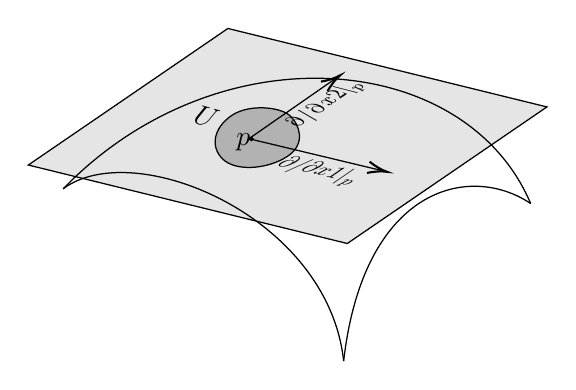
\begin{tikzpicture}[scale=0.85, x=0.75pt,y=0.75pt,yscale=-1,xscale=1]
%uncomment if require: \path (0,360); %set diagram left start at 0, and has height of 360

%Shape: Rectangle [id:dp08691604933838892] 
\draw  [fill={rgb, 255:red, 229; green, 229; blue, 229 }  ,fill opacity=1 ] (193.4,31.09) -- (374.22,75.57) -- (261.08,152.98) -- (80.26,108.5) -- cycle ;
%Shape: Polygon Curved [id:ds13972230036871047] 
\draw  [fill={rgb, 255:red, 178; green, 178; blue, 178 }  ,fill opacity=1 ] (195.67,80.33) .. controls (205.67,73.67) and (223,75.67) .. (228.33,80.33) .. controls (233.67,85) and (238.33,96.33) .. (227,103.67) .. controls (215.67,111) and (197.67,112.33) .. (190.33,105) .. controls (183,97.67) and (185.67,87) .. (195.67,80.33) -- cycle ;
%Curve Lines [id:da3913670271390508] 
\draw    (100,122) .. controls (140,92) and (250.33,137.67) .. (259,219.67) ;
%Curve Lines [id:da7387351338025494] 
\draw    (100,122) .. controls (188.33,31) and (328.33,43.67) .. (365,130.33) ;
%Curve Lines [id:da8758985242679558] 
\draw    (259,219.67) .. controls (270.33,121) and (330.33,107) .. (365,130.33) ;
%Shape: Circle [id:dp9796756156419224] 
\draw  [fill={rgb, 255:red, 0; green, 0; blue, 0 }  ,fill opacity=1 ] (205.67,93.67) .. controls (205.67,93.11) and (206.11,92.67) .. (206.67,92.67) .. controls (207.22,92.67) and (207.67,93.11) .. (207.67,93.67) .. controls (207.67,94.22) and (207.22,94.67) .. (206.67,94.67) .. controls (206.11,94.67) and (205.67,94.22) .. (205.67,93.67) -- cycle ;
%Straight Lines [id:da8885224032682308] 
\draw    (204.99,93.82) -- (255.36,58.81) ;
\draw [shift={(257,57.67)}, rotate = 145.2] [color={rgb, 255:red, 0; green, 0; blue, 0 }  ][line width=0.75]    (10.93,-3.29) .. controls (6.95,-1.4) and (3.31,-0.3) .. (0,0) .. controls (3.31,0.3) and (6.95,1.4) .. (10.93,3.29)   ;
%Straight Lines [id:da022213529301427393] 
\draw    (205.67,93.67) -- (281.67,111.88) ;
\draw [shift={(283.61,112.35)}, rotate = 193.48] [color={rgb, 255:red, 0; green, 0; blue, 0 }  ][line width=0.75]    (10.93,-3.29) .. controls (6.95,-1.4) and (3.31,-0.3) .. (0,0) .. controls (3.31,0.3) and (6.95,1.4) .. (10.93,3.29)   ;

% Text Node
\draw (196.67,89.4) node [anchor=north west][inner sep=0.75pt]    {$p$};
% Text Node
\draw (177.02,73.02) node [anchor=north west][inner sep=0.75pt]  [rotate=-15.82,xslant=0.18]  {$U$};
% Text Node
\draw (229.85,100.72) node [anchor=north west][inner sep=0.75pt]  [font=\scriptsize,rotate=-13.8,xslant=0.89]  {$\partial /\partial \sub x{1} |_{p}$};
% Text Node
\draw (219.33,84.95) node [anchor=north west][inner sep=0.75pt]  [font=\scriptsize,rotate=-326.11,xslant=-0.89]  {$\partial /\partial \sub x{2} |_{p}$};


\end{tikzpicture}

	\caption{Espaço Tangente}
\end{figure}

Outro conceito muito importante é o de diferencial de uma função suave. Se $F: N \longrightarrow M$ é uma função $C^\infty$, chamamos de \textit{diferencial} num ponto $p$ o mapa
\[
F_*: T_pN \longrightarrow T_{F(p)}M
\]
definido do seguinte modo: Se $X_p \in T_pN$, então $F_*(X_p) \in T_pM$ é dado por
\[
(F_*(X_p))f = X_p(f \circ F),
\]
onde $f \in C^{\infty}_{F(p)}(M)$. Se for preciso ressaltar o ponto $p$ (mas só se for realmente necessário), denotaremos $F_*$ por $F_{*,p}$.

\begin{teorema}[Regra da Cadeia]\label{reo: regra da cadeia}
	Se $F: N \longrightarrow M$ e $G: M \longrightarrow P$ são mapas suaves entre variedades e $p \in N$, então $(G \circ F)_{*,p} = G_{*,F(p)} \circ F_{*,p}$.
\end{teorema}

É fácil ver que a diferencial da identidade é a própria identidade no espaço tangente. Assim, utilizando a Regra da Cadeia \ref{reo: regra da cadeia}, a diferencial possui uma propriedade ``funtorial''. Com essas observações, não é difícil provar o seguinte resultado bastante natural:

\begin{proposicao}
	Se $F: N \longrightarrow M$ é um difeomorfismo entre variedades e $p \in N$, então $F_*: T_{F(p)}N \longrightarrow T_pM$ é um isomorfismo de espaços vetoriais.
\end{proposicao}

\subsection{Formas diferenciais}

Um $k$-\textit{tensor} num espaço vetorial $V$ é uma função $k$-linear de $V \times \dotsb \times V$ ($k$ vezes) em $\R$. Um $k$-tensor é \textit{alternado} se, ao trocarmos duas coordenadas de posição, o valor do tensor troca de sinal. Estudaremos $k$-tensores definidos no espaço tangente a uma variedade. A ideia é que esses tensores dão a noção de volume, assim como o determinante (que é um tensor) nos dá o volume de paralelepípedos em $\R^n$. Denotaremos o conjunto dos $k$-tensores alternados em $V$ por $A_k(V)$.

\begin{definicao}
	Uma $k$-\textit{forma} $\omega$ numa variedade $M$ é uma função que associa a cada ponto $p \in M$ um $k$-tensor alternado $\omega_p \in A_k(T_pM)$.
\end{definicao}

Será importante trabalhar com $0$-formas, e uma $0$-forma em $M$ nada mais é do que uma função de $M$ em $\R$ (cada ponto é associado a um $0$-tensor, que seria um ponto de $\R$).

\begin{exemplo}[Exemplo canônico de uma $1$-forma] 
	Se $(U,\phi)$ é uma carta coordenada numa variedade em $M$ e se $\sub x1,\dots,x_n$ são suas coordenadas, podemos definir
	\[
	(\de{x_n})_p(X_p) = X_p(x_n)
	\]
	para $p \in U$ e $X_p \in T_pM$. É imediato que $(\de{x_n})_p$ é uma função linear de $T_pM$ em $\R$, de modo que $\de{x_n}$ é uma $1$-forma em $U$. Note que $A_1(T_pM)$ é o espaço dual de $T_pM$ e é possível mostrar que $(\de{\sub x1})_p, \ldots, (\de{x_n})_p$ formam uma base de $A_1(T_pM)$ dual à base $\partial/\partial \sub x1|_p, \ldots ,\partial/\partial x_n|_p$ de $T_pM$.
\end{exemplo}

O exemplo anterior pode ser generalizado para $k$-formas. Denote por $\mathfrak S_n$ o conjunto das permutações do conjunto dos índices $1,\ldots,n$. Se $v=(\sub v1,\ldots,v_n)$ e $\sigma$ uma permutação, defina $v^\sigma = (v_{\sigma(1)},\ldots, v_{\sigma(n)})$. 

\begin{definicao}
	Se $\alpha$ é um $k$-tensor alternado e $\beta$ é um $\ell$-tensor alternado em $V$, podemos definir o seu \textit{produto exterior}, que é o $(k+\ell)$-tensor alternado $\alpha \wedge \beta$ dado por
	\[
	(\alpha \wedge \beta)(u,v) = \frac{1}{k!\ell!}\sum_{\sigma \in \mathfrak S_{k+\ell}} \sgn\sigma\alpha(u^\sigma)\beta(v^\sigma),
	\]
	onde $\sigma$ percorre todas as permutações dos números de $1$ até $k+\ell$ e $\sgn{\sigma}$ denota o \textit{sinal} da permutação $\sigma$.
\end{definicao}

É importante ressaltar que o produto exterior é associativo e anticomutativo. Nesse sentido, se $\omega$ é uma $k$-forma e $\tau$ é uma $\ell$-forma em $M$, então seu produto exterior é definido ponto a ponto:
\[
(\omega \wedge \tau)_p = \omega_p \wedge \tau_p.
\]

Um resultado interessante é que, sobre uma carta coordenada $(U,\phi)$ com componentes $\sub x1,\dots,x^n$, uma base para $A_k(T_pM)$ é dada pelos tensores
\[
(\de{x_{i_1}})_p \wedge \dotsb \wedge (\de{x_{i_k})}_p, \quad 1 \leq i_1 < \dotsb < i_k \leq n.
\]
Assim, toda $k$-forma $\omega$ em $U$ se escreve como
\[
\omega = \sum a_{i_1 \dotsb i_k} \de{x_{i_1}} \wedge \dotsb \wedge \de{x_{i_k}},
\]
onde $a_{i_1 \dotsb i_k}$ são funções em $U$. Com base nessa propriedade, diremos que uma $k$-forma $\omega$ em $M$ é \textit{suave}\footnote{Um jeito natural de definir a suavidade de uma $k$-forma é através do \textit{fibrado cotangente} da variedade, mas não entraremos nos detalhes dessa abordagem.} ou $C^{\infty}$ se em toda carta $(U, \phi)$ os coeficientes $a_{i_1 \dotsb i_k}$ acima forem funções $C^{\infty}$ em $U$. Denotaremos o conjunto de todas as $k$-formas $C^{\infty}$ em $M$ por $\Omega^k(M)$. Vale notar que $\Omega^0(M)$ é exatamente o conjunto das funções suaves de $M$ em $\R$. Também podemos considerar $\Omega^*(M)$ como sendo a soma direta dos espaços $\Omega^k(M)$ para $k \geq 0$.

Agora vamos definir duas operações muito importantes no estudo de formas: o \textit{pullback} e a derivada exterior. Se $T: V \longrightarrow W$ é uma transformação linear entre espaços vetoriais, temos o \textit{pullback} induzido $T^*: A_k(W) \longrightarrow A_k(V)$ dado por
\[
(T^*\alpha)(v_1,\dots,v_k) = \alpha(T(v_1),\dots,T(v_k))
\]
para $\alpha \in A_k(W)$ e $v_1,\dots,v_k \in V$. No contexto de espaços tangentes, se $F: N \longrightarrow M$ é um mapa $C^{\infty}$ entre variedades, para cada ponto $p \in N$ podemos tomar o \textit{pullback} da diferencial $F_{*,p}$:
\[
(F_{*,p})^*: A_k(T_{F(p)}M) \longrightarrow A_k(T_pN)
\]
Simplificaremos essa notação para $F^*$ apenas. Assim, se $\omega$ é uma $k$-forma em $M$, o seu \textit{pullback} é a $k$-forma $F^*\omega$ em $N$ dada por $(F^*\omega)_p = F^*(\omega_{_{F(p)}})$ para todo $p \in N$.

O \textit{pullback} de formas possui algumas propriedades importantes. Se $\omega$ é uma $k$-forma suave, então $F^*\omega$ também é suave. Além disso, visto como função de $\Omega^k(M)$ em $\Omega^k(N)$, o \textit{pullback} é linear. Outra propriedade importante é que ele ``comuta'' com o produto exterior, ou seja,
\[
F^*(\omega \wedge \tau) = F^*(\omega) \wedge F^*(\tau).
\]
Por fim, temos mais uma propriedade funtorial importante: $(G \circ F)^* = F^* \circ G^*$, para mapas suaves $F: N \longrightarrow M$ e $G: M \longrightarrow P$ entre variedades.

Vejamos agora o que é a derivada exterior. Começamos com o conceito para uma $0$-forma. Se $f \in \Omega^0(M)$, sua \textit{diferencial} é a $1$-forma $\de f$ em $M$ dada por
\[
(\de f)_p(X_p) = X_p(f)
\]
para $p \in M$ e $X_p \in T_pM$. Note que a definição que demos para $\de{x_n}$ é exatamente a diferencial da função coordenada $x_n$. Com essa definição em mãos, é possível mostrar que existe uma única função linear $\operatorname{d}: \Omega^*(M) \longrightarrow \Omega^*(M)$ satisfazendo:
\begin{itroman}
	\item Se $\omega$ é uma $k$-forma, então $\de\omega$ é uma $(k+1)$-forma.
	\item Se $\omega$ é uma $k$-forma e $\tau$ uma $\ell$-forma, então\footnote{Essa é quase uma ``regra de Leibniz'' com um fator de sinal, que é herdado da anticomutatividade do produto exterior.} 
	\[
	\de{(\omega \wedge \tau)} = (\de\omega) \wedge \tau + (-1)^k \omega \wedge (\de\tau).
	\]
	\item $\operatorname{d}^2 = 0$.
	\item Se $f$ é uma $0$-forma, então $\de f$ é a diferencial de $f$ como definida acima.
\end{itroman}
Se $(U,\phi)$ é uma carta coordenada em $M$ com funções coordenadas $\sub x1,\dots,x^n$ e $\omega$ é uma $k$-forma em $U$, pode-se mostrar que
\[
\de\omega = \sum_{i_1 \dotsb i_k} \sum_j \frac{\partial a_{i_1 \dotsb i_k}}{\partial x^j} \de{x^j} \wedge \de{x_{i_1}} \wedge \dotsb \wedge \de{x_{i_k}},
\]
onde $a_{i_1 \dotsb i_k}$ são os coeficientes de $\omega$ escrita na ``base'' $\de{\sub x1}, \dots, \de{x^n}$. Outra propriedade digna de nota é que a derivada exterior ``comuta'' com o \textit{pullback}: se $F: N \longrightarrow M$ é um mapa suave entre variedades, então
\begin{equation*}
	\label{eq: pullback comuta}
	\de{(F^*\omega)} = F^*\de\omega
\end{equation*}
para qualquer $\omega \in \Omega^k(M)$.

\tagged{integracao}{
\subsection{Integração em variedades}
	Terminamos essa seção com uma breve descrição de como utilizar formas para integrar em variedades. Começamos com a integral em $\R^n$. Se $\omega = f(x) \,\de{\sub x1} \wedge \dotsb \wedge \de{x^n}$ é uma $n$-forma $C^{\infty}$ definida num aberto $U \subseteq \R^n$, sua integral sobre $U$ é definida pela Integral de Riemann de $f$:
	\[
	\int_U \omega = \int_U f(x) \,\de{\sub x1} \wedge \dotsb \wedge \de{x^n} \coloneqq \int_U f(x) \,\de{\sub x1}\dotsb \de{x^n},
	\]
	se a integral existir. A priori, parece que não estamos fazendo nada de novo, mas a linguagem de formas se comporta muito bem com a mudança de coordenadas. Se $T: \R^n \supseteq V \longrightarrow U \subseteq \R^n$ é um difeomorfismo que preserva orientação, então
	\[
	\int_V T^*\omega = \int_U \omega.
	\]
	É muito importante que o difeomorfismo anterior preserve orientação. Por causa disso, só conseguiremos integrar em variedades orientáveis\footnote{Uma variedade é \textit{orientável} se possui um atlas tal que a função de transição entre duas cartas quaisquer sempre preserva orientação, ou seja, tem determinante Jacobiano positivo.}.
	
	Finalmente, seja $M$ uma variedade orientada de dimensão $n$. Tome $\omega \in \Omega^n(M)$ de suporte compacto. Se o suporte de $\omega$ está contido numa carta coordenada $(U,\phi)$ do atlas orientado, definimos
	\[
	\int_U \omega \coloneqq \int_{\phi(U)}(\phi^{-1})^*\omega,
	\]
	que é a integral de uma forma em $\R^n$. Mostra-se que isso está bem-definido e não depende da carta escolhida. Caso não consigamos encontrar a carta $U$, ainda conseguimos definir a integral de $\omega$ para todo $M$ através de uma partição da unidade.
}

\subsection{Campos e Fibrados vetoriais}
Se voltarmos as aulas de cálculo e considerar um aberto $U\subset \R^n$, os campos suaves eram aplicações com a seguinte cara:
\begin{equation*}
	\function{{F}{U}{U\times \R^n}{x}{(x, f_1(x), \ldots, f_n(x))}}
\end{equation*}
de modo que a aplicação $(f_1,\ldots, f_n):U \longto \R^n$ era suave. Podemos reinterpretar essa noção através da projeção canônica da primeira coordenada $\Pi_1$, onde os campos suaves são as aplicações suaves $F: U \longto U\times \R^n$ tal que $\Pi_1 \circ F = \sub{\Id}{\R^n}$. Nesse contexto, o aberto $U$ é o nosso \textit{espaço de configurações} e o produto cartesiano $U\times \R^n$ o nosso \textit{espaço de fases}.

\begin{definicao}
	Sejam $E$ e $M$ variedades, $\pi: E \rightarrow M$ uma submersão. Suponha que existe uma cobertura $\left(U_\alpha\right)_{\alpha}$ de $M$ e difeomorfismos $\phi_\alpha: U_\alpha \times \mathbb{R}^n \longto \pi^{-1}\left(U_\alpha\right)$ tais que:
	\begin{itroman}
		\item $\pi \circ \phi_\alpha = \sub\Id M$.
		\item Se $U_\alpha$ e $U_\beta$ não são disjuntos, então 
		\begin{eqspaced*}{\begin{pmatrix} p\in U_\alpha \cap U_\beta\\ v \in \R^n\end{pmatrix}}
			\phi_\beta^{-1} \circ \phi_\alpha(p, v)=\left(p, \theta_{\beta, \alpha}(p) v\right)
		\end{eqspaced*}
		onde $\theta_{\alpha, \beta} : U_\alpha \cap U_\beta \longto \GL_n(\R)$ é suave.
		\item $\left(\phi_\alpha, U_\alpha\right)$ é máximo em relação aos itens acima.
	\end{itroman}
A tripla $(E, M, \pi)$ é chamada de \textit{fibrado vetorial} de posto $n$ e projeção $\pi$. Para cada $p \in M$ o espaço $E_p\coloneqq \pi^{-1}(p)$ é chamado \textit{fibra} sobre $p$ e herda naturalmente uma estrutura de espaço vetorial.
\end{definicao}

O espaço tangente já nos fornece dois exemplos importantes de fibrados: O \textit{fibrado tangete} $TM \coloneqq \bigcup_{p\in M} T_pM $ e o \textit{cotangente} $TM^* \coloneqq \bigcup_{p\in M} (T_pM)^* $ onde cada $(T_pM)^*$ é o espaço dual de $T_pM$.

\begin{figure}[H]
	\centering
	

\tikzset{every picture/.style={line width=0.45pt}} %set default line width to 0.75pt        

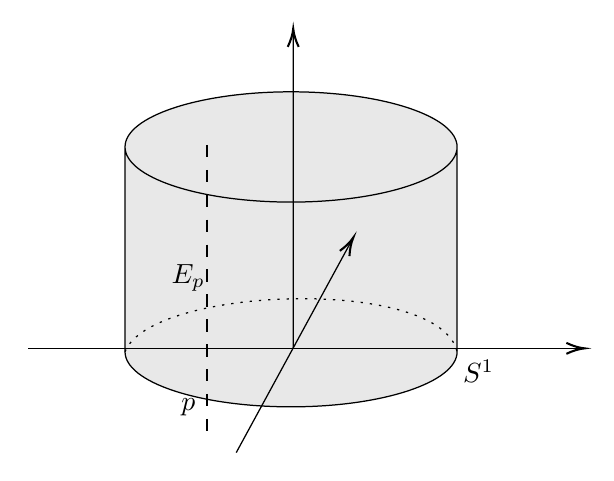
\begin{tikzpicture}[scale=0.8, x=0.75pt,y=0.75pt,yscale=-1,xscale=1]
%uncomment if require: \path (0,445); %set diagram left start at 0, and has height of 445

%Flowchart: Magnetic Disk [id:dp05785587446091456] 
\draw  [fill={rgb, 255:red, 232; green, 232; blue, 232 }  ,fill opacity=1 ] (298.5,110.04) -- (298.5,233.36) .. controls (298.5,251.7) and (253.73,266.56) .. (198.5,266.56) .. controls (143.27,266.56) and (98.5,251.7) .. (98.5,233.36) -- (98.5,110.04)(298.5,110.04) .. controls (298.5,128.38) and (253.73,143.25) .. (198.5,143.25) .. controls (143.27,143.25) and (98.5,128.38) .. (98.5,110.04) .. controls (98.5,91.71) and (143.27,76.84) .. (198.5,76.84) .. controls (253.73,76.84) and (298.5,91.71) .. (298.5,110.04) -- cycle ;
%Straight Lines [id:da047201416380546535] 
\draw    (40.25,231.34) -- (373.25,231.34) ;
\draw [shift={(375.25,231.34)}, rotate = 180] [color={rgb, 255:red, 0; green, 0; blue, 0 }  ][line width=0.75]    (10.93,-3.29) .. controls (6.95,-1.4) and (3.31,-0.3) .. (0,0) .. controls (3.31,0.3) and (6.95,1.4) .. (10.93,3.29)   ;
%Straight Lines [id:da32140623967458537] 
\draw    (165.5,294.09) -- (235.04,166.34) ;
\draw [shift={(236,164.59)}, rotate = 118.56] [color={rgb, 255:red, 0; green, 0; blue, 0 }  ][line width=0.75]    (10.93,-3.29) .. controls (6.95,-1.4) and (3.31,-0.3) .. (0,0) .. controls (3.31,0.3) and (6.95,1.4) .. (10.93,3.29)   ;
%Curve Lines [id:da7976987955408381] 
\draw  [dash pattern={on 0.84pt off 2.51pt}]  (98.5,233.36) .. controls (114,193.84) and (288,187.84) .. (298.5,233.36) ;
%Straight Lines [id:da639687396341936] 
\draw    (199.75,231.34) -- (199.8,40.84) ;
\draw [shift={(199.8,38.84)}, rotate = 90.01] [color={rgb, 255:red, 0; green, 0; blue, 0 }  ][line width=0.75]    (10.93,-3.29) .. controls (6.95,-1.4) and (3.31,-0.3) .. (0,0) .. controls (3.31,0.3) and (6.95,1.4) .. (10.93,3.29)   ;
%Straight Lines [id:da5733655963811695] 
\draw  [dash pattern={on 4.5pt off 4.5pt}]  (147.8,108.8) -- (147.8,281.8) ;

% Text Node
\draw (130.8,260.24) node [anchor=north west][inner sep=0.75pt]    {$p$};
% Text Node
\draw (125,179.4) node [anchor=north west][inner sep=0.75pt]    {$E_{p}$};
% Text Node
\draw (300.5,236.76) node [anchor=north west][inner sep=0.75pt]    {$S^{1}$};


\end{tikzpicture}
	\caption{Fibrado trivial de $S^1$}
\end{figure}

\begin{definicao}
	Uma \textit{seção} de um fibrado vetorial $(E,M,\pi)$ é uma aplicação $\xi : M \longto E$ tal que $\pi\circ \xi = \sub \Id M$. Em particular, um \textit{campo vetorial} $F$ é uma seção do fibrado tangente $TM$. O conjunto dos campos vetoriais de $M$ é denotado por $\mathfrak X(M)$ e é um módulo. 
\end{definicao}

\subsection{Métricas Riemannianas}

\begin{definicao}
	Uma \textit{métrica Riemanniana} de uma variedade $M$ é uma seção suave do fibrado dos 2-tensores simétricos positivos definidos em $TM$. Em outras palavras é uma aplicação que associa a cada ponto $p$ da variedade $M$ um produto interno $\mathrm{g}_p$ de $T_p M$ tal que $\mathrm{g}_{i, j}:=\mathrm{g}\left(\frac{\partial}{\partial x_i}, \frac{\partial}{\partial x_j}\right)$ é suave. Uma variedade $M$ com uma métrica $\mathrm g$ é chamada então de variedade Riemanniana.
\end{definicao}

Escrevendo em coordenadas, podemos considerar
\begin{equation*}
	\mathrm g \coloneqq \sum_{i,j} \mathrm g_{ij}\,\de x_i \otimes \de x_j.
\end{equation*}

Utilizando partições da unidade, sempre é possível considerar uma métrica riemanniana em qualquer variedade, induzida pela métrica euclidiana em cada carta coordenada. Isso é uma particularidade da métrica riemanniana em relação a outras estruturas geométricas (e.g. Lorentziana, simplética).